\documentclass[3p]{elsarticle}
\usepackage{graphicx,pst-all}
\usepackage{epstopdf}
\usepackage{multirow}
\usepackage{xspace}
\usepackage{tabularx}
\usepackage{rotating}
\usepackage{float}
\usepackage{amsmath,amssymb,pifont}
\usepackage[mathscr]{eucal}
\usepackage[english,french]{babel}
\usepackage[T1]{fontenc}
\usepackage[utf8]{inputenc}
\usepackage{hyperref}
\usepackage{dirtree}

\newcommand{\n}{\tabularnewline}
\newcolumntype{C}{>{\centering}X}
\newcolumntype{R}{>{\raggedleft}X} 
\newcolumntype{L}{>{\raggedright}X} 
\newcolumntype{M}[1]{>{\centering}m{#1}}

\newenvironment{legend}%
 {\tabular{r>{\small} l}}%
 {\endtabular}

\newcommand{\Rm}[1]{{\bf R}_{#1}^{g+}}
\newcommand{\Rr}[1]{{\bf r}_{#1}^{g\ast}}
\newcommand{\Sm}[1]{{S_{#1}^{g+}}}
\newcommand{\Sr}[1]{{s_{#1}^{g\ast}}}
\newcommand{\Nr}[1]{N_{#1}^{\ast}}
\newcommand{\M}{\mathbb}
\newcommand{\B}[1]{{\bf #1}\xspace}
\newcommand{\T}{\texttt}
\newcommand{\Mc}{\mathcal}
\newcommand{\Hi}{\textit}
\newcommand{\norm}[1]{\left\|#1\right\|}
\newcommand{\abs}[1]{\left|#1\right|}
\newcommand{\snorm}[1]{\|#1\|}
\newcommand{\psca}[2]{\left\langle #1 , #2 \right\rangle}
\newcommand{\pscac}[2]{\textcolor{red}{\left\langle \textcolor{black}{#1} , \textcolor{black}{#2} \right\rangle}}
\newcommand{\la}{\Big\langle}
\newcommand{\ra}{\Big\rangle}
\newcommand{\im}{{\bf i}\xspace}
\newcommand{\sg}{\textrm{sg}}

\newcommand{\Eq}[1]{Eq.~\ref{eq:#1}}
\newcommand{\Eqs}[2]{Eqs.~\ref{eq:#1} et~\ref{eq:#2}}
\newcommand{\Eqss}[3]{Eqs.~\ref{eq:#1},~\ref{eq:#2} and~\ref{eq:#3}}
\newcommand{\Fig}[1]{Figure~\ref{fig:#1}}
\newcommand{\Figs}[2]{Figures~\ref{fig:#1} et~\ref{fig:#2}}
\newcommand{\Figss}[3]{Figures~\ref{fig:#1},~\ref{fig:#2} et~\ref{fig:#3}}
\newcommand{\Tab}[1]{Tableau~\ref{tab:#1}}
\newcommand{\Tabs}[2]{Tableaux~\ref{tab:#1} et~\ref{tab:#2}}
\newcommand{\Tabss}[3]{Tableaux~\ref{tab:#1},~\ref{tab:#2} et~\ref{tab:#3}}
\newcommand{\Sect}[1]{\S~\ref{sect:#1}}
\newcommand{\Sects}[2]{\S~\ref{sect:#1}~et~\ref{sect:#2}}
\newcommand{\Sec}[1]{\Sect{#1}}
\newcommand{\App}[1]{Annexe~\ref{app:#1}}
%\renewcommand{\emph}[1]{\textcolor{red}{\bf #1}}

\newenvironment{remark}[1][\textit{Nota Bene}]{\begin{trivlist}
\item[\hskip \labelsep {\bfseries \rule{1ex}{1ex} #1}]\ignorespaces}{\rule{1ex}{1ex} \end{trivlist}\ignorespacesafterend}

\newcounter{question}
\newcommand{\Q}[1]{\stepcounter{question}\begin{remark}[Q\arabic{question}]#1~~\end{remark}}

% notations
\newcommand{\functional}[2][\cdot]{\mathbb{#2}\left[#1\right]}
\newcommand{\function}[2][\cdot]{#2\left(#1\right)}
\newcommand{\grad}[1]{\nabla #1}
\newcommand{\dX}[1]{\frac{\partial #1}{\partial x}}
\renewcommand{\div}[1]{\nabla \cdot #1}
\newcommand{\Lapl}[1]{\Delta #1}
\newcommand{\LaplX}[1]{\frac{\partial^2 #1}{\partial x^2}}
\newcommand{\domain}[1]{V_{#1}}
\newcommand{\boundary}[1]{\partial \domain{#1}}
\newcommand{\interface}[1]{\Gamma_{#1}}
\DeclareMathOperator*{\argmin}{arg\,min}

\addto\captionsenglish{%
  \renewcommand{\abstractname}{Description}
}
\addto\captionsfrench{%
  \renewcommand{\abstractname}{Description}
}

\newenvironment{abstracts}
 {\global\setbox\absbox=\vbox\bgroup
    \hsize=\textwidth
    \linespread{1}\selectfont}
 {\vspace{-\bigskipamount}\egroup}
\renewenvironment{abstract}[1][]
 {\if\relax\detokenize{#1}\relax\else\selectlanguage{#1}\fi
  \noindent\textbf{\abstractname}\par\medskip\noindent\ignorespaces}
 {\par\bigskip}

 
\raggedbottom

\makeatletter
\def\ps@pprintTitle{
      \let\@oddhead\@empty
      \let\@evenhead\@empty
      \def\@oddfoot{\reset@font\hfil\thepage\hfil}
      \let\@evenfoot\@oddfoot
}
\makeatother
\bibliographystyle{elsarticle-num}

\begin{document}

\begin{frontmatter}

\title{TD: modélisation transitoire d'un bain de corium en fond de cuve et évaluation du risque de percement de la cuve}

% \author[LMAG]{R.~Le Tellier\corref{contact}}
% \ead{romain.le-tellier@cea.fr}
% \cortext[contact]{contact:}
% 
% \address[LMAG]{CEA, DEN, DTN/SMTA/LMAG, Cadarache \\
%   F-13108 Saint Paul-lez-Durance, France}
  
\begin{abstracts}
\selectlanguage{french}
\begin{abstract}[french]
%   Resum\'e en fran\c{c}ais
Dans ce TD, on se propose d'étudier les résultats donnés par des calculs PROCOR modélisant un bain de corium en fond de cuve. Via différentes coulées provenant de la fonte, d'une part, des structures internes du réacteur et, d'autre part, de la fonte  de la cuve du réacteur, la thermochimie et la thermique du bain évoluent de manière transitoire dans le fond de cuve et cette évolution a un impact sur la charge thermique imposée sur la cuve du réacteur. On se propose d'étudier différents cas de test transitoires (différents instants de coulées et différentes options de modélisation dans le bain) correspondant à un benchmark proposé dans le cadre du projet européen H2020 IVRM \cite{Carenini2019} se basant sur l'étude d'accidents graves dans un réacteur type AP1000 \cite{Esmaili2004}. La stationnaire atteint pour chacun de ces cas de test est comparable au stationnaire en fond de cuve atteint dans le TD1.

Dans un premier temps, il s'agira de comprendre les différents cas de test proposés et l'impact des coulées et des options de modélisation sur le transitoire en fond de cuve puis de comparer le bilan thermique transitoire du bain au bilan thermique stationnaire fait pour le TD1. Dans un second temps, une étude statistique de sensibilités permettra d'identifier les paramètres de modélisation pouvant avoir un impact important sur la charge thermique imposée sur la cuve pouvant mener à son percement.
\end{abstract}
% \selectlanguage{english}
% \begin{abstract}
% %   Abstract in English 
% \end{abstract}
\end{abstracts}
  
\end{frontmatter}

\selectlanguage{french}

\section{Étude des cas de test du benchmark}

\subsection{Présentation des cas de test}
Les cas 1,2 et 3 du benchmark sont présentés dans la Fig.~\ref{fig:TD_benchmark}. Pour chacun des cas, différentes coulées et différentes options de modélisation sont choisies.
\begin{figure}[H]
  \centering 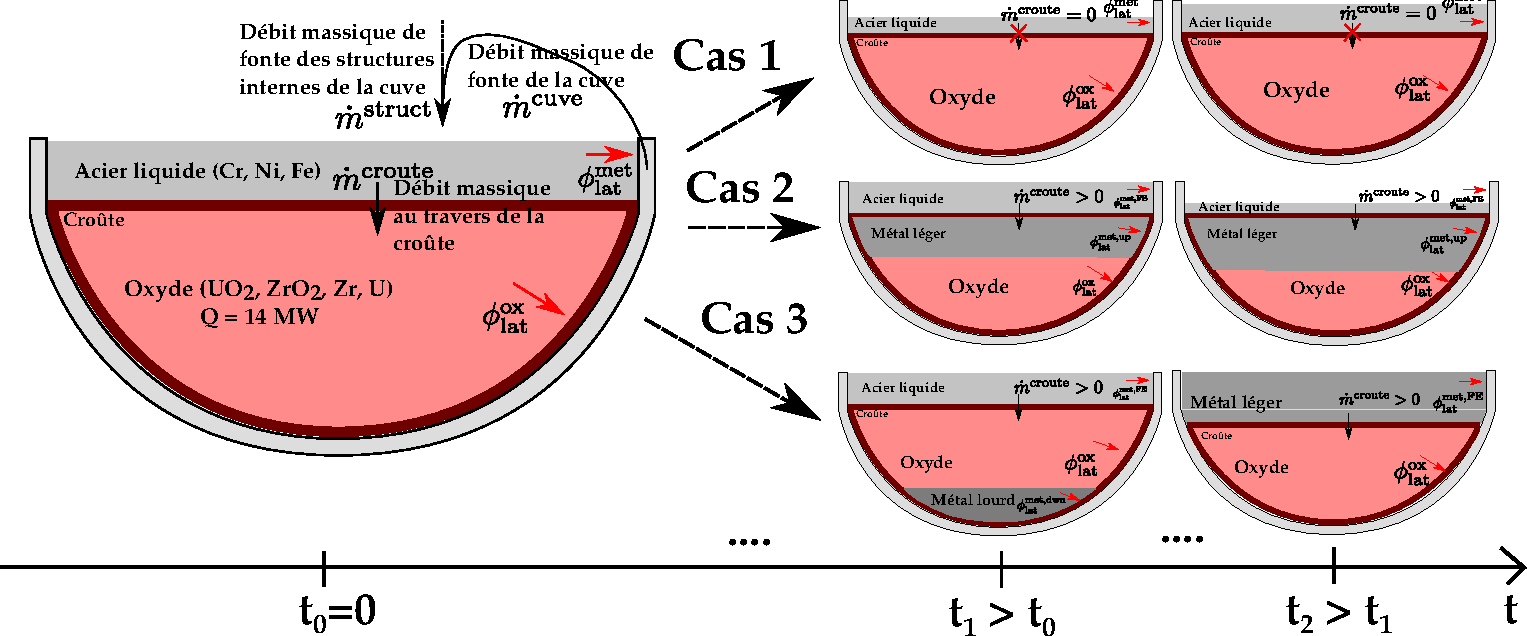
\includegraphics[width=\textwidth]{../Figures/TD_benchmark.pdf}
	\label{fig:TD_benchmark}
  \caption{Configurations initiale ($t_0$) et durant le transitoire ($t_1$ et $t_2$) pour les cas 1, 2 et 3 du benchmark.}
\end{figure} Dans tous les cas, la configuration initiale correspond à un bain oxyde en dessous d'une couche d'acier liquide. Un transfert radiatif (avec une émissivité $\epsilon$) par la surface supérieure de la couche d'acier liquide est imposé comme condition limite supérieure de cette couche. En plus des coulées `extérieures` correspondant à la fonte des structures internes du réacteur, des coulées $\dot{m}^{\text{cuve}}$ associées à l'ablation de la cuve par le bain de corium sont ajoutées au bain de corium et viennent modifier son inventaire en espèces chimiques.

Les conditions initiales à $t_0$ sont :
\begin{itemize}
	\item Masse de la couche oxyde :
	\begin{itemize}
		\item \emph{Cas n$^{\circ}$1 :} mUO$_2$ = 59.6t,  mZR = 6.58t, mZRO$_2$ = 15t
		\item \emph{Cas n$^{\circ}$2 et 3 :} mUO$_2$ = 68t,  mZR = 7.5t, mZRO$_2$ = 17t
	\end{itemize}
	\item Masse de la couche d'acier liquide :
	\begin{itemize}
		\item \emph{Cas n$^{\circ}$1:} mCr = 7.2t,  mNi = 2.7t, mFe = 27.7t
		\item \emph{Cas n$^{\circ}$2:} mCr = 5.7t,  mNi = 2.2t, mFe = 22.1t	
		\item \emph{Cas n$^{\circ}$3:} mCr = 1.9t,  mNi = 0.7t, mFe = 7.4t
	\end{itemize}
\end{itemize}

Le transfert de masse par thermochimie au travers de la croûte horizontale, $\dot{m}^{\text{croûte}}$, peut ou non être activé :
\begin{itemize}
	\item \emph{Cas n$^{\circ}$1 :} $\dot{m}^{\text{croûte}} = 0$
	\item \emph{Cas n$^{\circ}$2 et 3 :} $\dot{m}^{\text{croûte}} > 0$
\end{itemize}

Des coulées $\dot{m}^{\text{struct}}$, corresondant à la fonte des éléments du réacteur arrivant dans le bain, différentes sont considérées : 
\begin{itemize}
	\item \emph{Cas n$^{\circ}$1, 2 et 3:} $\dot{m}^{\text{struct}}(t) = 6\text{kg.s}^{-1} \text{ pour } 6000\leq t\leq 9000$
	\item \emph{Cas n$^{\circ}$3:} $\dot{m}^{\text{struct}}(t) = 5\text{kg.s}^{-1} \text{ pour } 800\leq t\leq 4800$
\end{itemize}

La stratification du bain de corium peut ou non être calculée : 
\begin{itemize}
		\item \emph{Cas n$^{\circ}$1 et 2:} pas de stratification dans le bain sous la croûte, une seule couche oxyde;
		\item \emph{Cas n$^{\circ}$3:} stratification du bain en \emph{métal lourd/oxyde} suite à la 1\iere{} coulée puis en \emph{oxyde/métal léger} suite à la 2\ieme{} coulée.
\end{itemize}

\subsection{Lancement et analyse des cas de test}
Arborescence du répertoire de travail pour le TD2 :
\dirtree{%
.1 .
.2 benchmarkLauncher.sh.
.2 appScilab.sh.
.2 data.
.3 vessel\_steel\_properties/.
.3 ap1000\_lower\_head\_application\_parameter\_input\_file.txt.
.3 ap1000\_benchmark\_parameter\_input\_file.txt.
.2 output.
}
Les différents fichiers correspondent à :
\begin{itemize}
	\item \texttt{benchmarkLauncher.sh} : \emph{script de lancement du benchmark PROCOR} utilisant l'application fond de cuve PROCOR pour chaque cas de test;
	\item \texttt{appScilab.sh} : \emph{script de lancement de l'outil Scilab} permettant de tracer les courbes des sortes PROCOR;
	\item \texttt{vessel\_steel\_properties} : propriétés physique de l'acier de cuve;
	\item \texttt{ap1000\_lower\_head\_appication\_parameter\_input\_file.txt} : fichier d'entrées de l'application fond de cuve PROCOR dans lequel les différentes options de modélisation peuvent être modifiées;
	\item \texttt{ap1000\_benchmark\_parameter\_input\_file.txt} : fichier d'entrées du benchmark permettant de surcharger des entées de l'application fond de cuve et/ou du benchmark. C'est celui utilisé pour l'étude statistique pour faire varier des paramètres aléatoirement;
	\item les sorties seront dans \texttt{output}.
\end{itemize}
Les cas de test du benchmark peuvent être lancés via :
\begin{itemize}
\item \texttt{./benchmarkLauncher.sh AP1000Benchmark data/ ap1000\_benchmark\_parameter\_input\_file.txt output/}
\end{itemize}
Les sorties PROCOR dans \texttt{output/} sont :
\begin{itemize}
\item des fichiers \texttt{*.csv} contenant les données temporelles des différents modèles de l'application fond de cuve;
\item des fichiers \texttt{*.png} permettant une visualisation `grossière` du fond de cuve au cours du temps;
\item des fichiers \texttt{VTK/*.vtk} permettant une visualisation à l'aide du logiciel PARAVIEW;
\end{itemize}
Elles peuvent être analysées via l'outil Scilab. Celui ci peut être lancé via :
\begin{itemize}
\item \texttt{./appScilab.sh -aTransientInLowerHead masses temperatures ...}
\item Les arguments \texttt{masses temperatures ...} indiquent au script les courbes à tracer. Les courbes disponibles sont : \texttt{masses, mass\_fractions, heights, temperatures, powers, heat\_fluxes, vessel, water}
\end{itemize}

\subsection{Étude du cas 1}
\Q{Observer et expliquer le transitoire de $\bar{\phi}^{oxy}_{up}$, le flux de chaleur moyen par la surface supérieure du bain oxyde.}
\Q{Observer et expliquer le transitoire de $T_{met,FE}^{liq}$, la température moyenne de la couche d'acier liquide.}
\Q{Observer et expliquer le transitoire de l'épaisseur $h^{liq.}_{met,FE}$ de la couche d'acier liquide.}
\Q{Expliquer le transitoire de $\bar{\phi}^{met,FE}_{lat}$, le flux de chaleur moyen par la surface latérale de la couche d'acer liquide.}
\Q{Expliquer l'augmentation de $h^{liq.}_{met,FE}$ lorsque $\bar{\phi}^{met,FE}_{lat}$ augmente.}
À ce stade, il est important de comprendre l'intéraction entre $h^{liq.}_{met,FE}$ et $\bar{\phi}^{met,FE}_{lat}$.
\Q{Expliquer le transitoire des flux de chaleur imposés à différentes altitudes (notée $z$) de la paroie interne de la cuve et leur impact sur l'épaisseur de la cuve.}
Suites à ces questions, le temps auquel le flux de chaleur par la surface latérale de la couche d'acier liquide sera maximal peut être déduit.
\Q{Relever graphiquement cette valeur et la comparer au flux stationnaire $\phi^{met}_{lat}$ calculé au TD1.}
\Q{Dans le fichier d'entrées du benchmark, faire varier l'émissivité de la couche d'acier liquide. Expliquer son impact sur le focusing effect.}

\subsection{Étude du cas 2 et 3}
Pour ces cas, les coulées venant des structures internes du réacteur ainsi que les options de modélisation sont différentes. Le transitoire suivi par le bain de corium ainsi que le transitoire d'ablation de la cuve sont donc différents.

\Q{En suivant le même démarche que pour le cas 1, expliquer le flux maximal imposé par la couche d'acier liquide.}
\Q{Relever ce flux maximal et le comparer au flux stationnaire calculer lors du TD1.}

\section{Étude statistique}

\section*{Références}

\bibliography{../lma-jabref.bib}

\end{document}
